\documentclass[xcolor=dvipsnames,t]{beamer} 

\usepackage{listings} 
\usepackage{color} 
\usepackage{xcolor}  
\usepackage{microtype} 
\usepackage{helvet} 
\usepackage{inconsolata} 
\usepackage[framemethod=TikZ]{mdframed} 
\usepackage{graphicx} 
\usepackage{alltt}
\usepackage{sverb} 
\usepackage{verbatim} 

%%% This is the automatic preamble used by IPython.  Note that it does *not*
%% include a documentclass declaration, that is added at runtime to the overall
%% document.

\usepackage{amsmath}
\usepackage{amssymb}
\usepackage{graphicx}

% needed for markdown enumerations to work
\usepackage{enumerate}

% Slightly bigger margins than the latex defaults
\usepackage{geometry}
\geometry{verbose,tmargin=3cm,bmargin=3cm,lmargin=2.5cm,rmargin=2.5cm}

% Define a few colors for use in code, links and cell shading
\usepackage{color}
\definecolor{orange}{cmyk}{0,0.4,0.8,0.2}
\definecolor{darkorange}{rgb}{.71,0.21,0.01}
\definecolor{darkgreen}{rgb}{.12,.54,.11}
\definecolor{myteal}{rgb}{.26, .44, .56}
\definecolor{gray}{gray}{0.45}
\definecolor{lightgray}{gray}{.95}
\definecolor{mediumgray}{gray}{.8}
\definecolor{inputbackground}{rgb}{.95, .95, .85}
\definecolor{outputbackground}{rgb}{.95, .95, .95}
\definecolor{traceback}{rgb}{1, .95, .95}
\definecolor{inputbg}{rgb}{0.98, 0.98, 0.98}

% Framed environments for code cells (inputs, outputs, errors, ...).  The
% various uses of \unskip (or not) at the end were fine-tuned by hand, so don't
% randomly change them unless you're sure of the effect it will have.
\usepackage{framed}

% remove extraneous vertical space in boxes
\setlength\fboxsep{0pt}

% codecell is the whole input+output set of blocks that a Code cell can
% generate.
\newenvironment{codecell}{%
    \def\FrameCommand{\color{mediumgray} \vrule width 1pt \hspace{5pt}}%
   \MakeFramed{\vspace{-0.5em}\FrameRestore}}
 {\unskip\endMakeFramed}

 \newenvironment{codeinput}{%
   \def\FrameCommand{\colorbox{inputbg}}%
   \MakeFramed{\advance\hsize-\width \FrameRestore}}
 {\unskip\endMakeFramed}

\newenvironment{codeoutput}{%
   \def\FrameCommand{\colorbox{outputbackground}}%
   \vspace{-1.4em}
   \MakeFramed{\advance\hsize-\width \FrameRestore}}
 {\unskip\medskip\endMakeFramed}

\newenvironment{traceback}{%
   \def\FrameCommand{\colorbox{traceback}}%
   \MakeFramed{\advance\hsize-\width \FrameRestore}}
 {\endMakeFramed}

% Use and configure listings package for nicely formatted code
\usepackage{listings}
\lstset{
  %numbers=left,
  language=python,
  aboveskip=\smallskipamount,
  belowskip=\smallskipamount,
  xleftmargin=3mm,
  breaklines=true,
  basicstyle=\small \ttfamily,
  showstringspaces=false,
  keywordstyle=\color{blue}\bfseries,
  commentstyle=\color{myteal},
  stringstyle=\color{darkgreen},
  %identifierstyle=\color{darkorange},
}

% The hyperref package gives us a pdf with properly built
% internal navigation ('pdf bookmarks' for the table of contents,
% internal cross-reference links, web links for URLs, etc.)
\usepackage{hyperref}
\hypersetup{
  breaklinks=true,  % so long urls are correctly broken across lines
  colorlinks=true,
  urlcolor=blue,
  linkcolor=darkorange,
  citecolor=darkgreen,
  }

% hardcode size of all verbatim environments to be a bit smaller
\makeatletter 
\g@addto@macro\@verbatim\small\topsep=0.5em\partopsep=0pt
\makeatother 

% Prevent overflowing lines due to urls and other hard-to-break entities.
\sloppy

\usepackage[framemethod=TikZ]{mdframed} 
\usepackage{lipsum} 
\usepackage{microtype} 
%\usepackage{mathptmx} 
\usepackage{pifont} 
\usepackage{graphicx} 

\usepackage{listings} 
\lstset{language=python, 
        %basicstyle=\footnotesize\ttfamily, 
        basicstyle=\small\ttfamily,
        columns=fullflexible, 
        %title=\lstname, 
        %numbers=left, stringstyle=\texttt, 
        %numberstyle={\tiny\texttt}, 
        keywordstyle=\color{blue}, 
        commentstyle=\color{darkgreen}, 
        stringstyle=\color{purple} } 

\lstdefinestyle{json}{
        language=python, 
        basicstyle=\tiny\ttfamily,
        columns=fullflexible, 
        %title=\lstname, 
        %numbers=left, stringstyle=\texttt, 
        %numberstyle={\tiny\texttt}, 
        keywordstyle=\color{blue}, 
        commentstyle=\color{darkgreen}, 
        stringstyle=\color{purple}
}


\mdfsetup{skipabove=\topskip, skipbelow=\topskip} 

\definecolor{codebg}{rgb}{0.99,0.99,0.99}
\definecolor{darkgreen}{rgb}{0.0, 0.5, 0.0}

\global\mdfdefinestyle{code}{%
    frametitlerule=true,%
    frametitlefont=\small\bfseries\ttfamily,%
    frametitlebackgroundcolor=lightgray,%
    backgroundcolor=codebg,%
    linecolor=gray, linewidth=0.5pt,%
    leftmargin=0.5cm, rightmargin=0.5cm,%
    roundcorner=2pt,%
    innerleftmargin=5pt
}

\global\mdfdefinestyle{code2}{%
    topline=false,%
    bottomline=false,%
    leftline=true,%
    rightline=false,%
    backgroundcolor=codebg,%
    linecolor=gray, linewidth=0.5pt,%
    leftmargin=0.0cm, rightmargin=0.0cm,%
    innerleftmargin=1pt
}


 

\title[Intelligent Agents in Virtual Environments]{Intelligent Agents in Virtual Environments} 

\subtitle{Designing Virtual Environments for Artificial Intelligence in
Computational Simulations and Video Games} 

\author[Michael Papasimeon]{Dr Michael Papasimeon \\[0.2in] 
                Guest Lecture\\
                Graphics and Interaction\\} 
\date{10 October 2014}

\subject{Talks} 

%\usetheme{Rochester} 
%\usetheme{Warsaw} 
%\usetheme{Berkeley} 
%\usetheme[compress]{Berlin} 
%\usetheme{Frankfurt} 
%\usetheme{Darmstadt} 
%\usetheme{Boadilla} 
\usetheme{Madrid} 
%\usetheme{AnnArbor} 
%\usetheme{CambridgeUS} 
%\usetheme{Marburg} 
%\usetheme{Malmoe} 
%\usetheme{Antibes} 
%\usetheme{default} 
%\usecolortheme[named=Red]{structure}
%\usecolortheme{dove} 
\setbeamertemplate{navigation symbols}{}
\setbeamertemplate{blocks}[default]
%\usefonttheme{structurebold} 


\begin{document}

\begin{frame}
    \titlepage
\end{frame} 

\begin{frame}{Introduction} 
So what is this lecture all about? \\[1cm] 
\begin{block}{In general...}   
Where \textbf{Artificial Intelligence} meets \textbf{Computer Graphics}
\end{block} 
\pause
\begin{block}{but more specifically...} 
The interaction between \textbf{Intelligent Agents} and \textbf{Virtual Environments}
\end{block} 
\end{frame} 

\begin{frame}{Definitions} 
    \begin{description}
        \item[Virtual Environment] a dynamic computational representation of a
        world~\footnote{Real, fictitious or abstract world} 
        populated by entities and intelligent agents. 
        \item[Intelligent Agents] an autonomous decision making entity situated
        in virtual environment that can perceive the environment, reason and
        make decisions and take action in the environment.  
    \end{description} 
\end{frame} 

\begin{frame}{Applications} 
\begin{itemize} 
    \item Computational Simulations
    \item Video Games
    \item Virtual Realities
\end{itemize} 
\vspace{0.5in} 
When these \emph{Virtual Environments} are populated with \emph{Intelligent
Agents} we often call these systems \emph{Multi-Agent Simulations} 
\end{frame} 

\begin{frame}{Agent--Environment Interaction} 
TODO: Figure showing Agent-Environment Interaction
Perception-Reasoning-Action Model 
\begin{center}
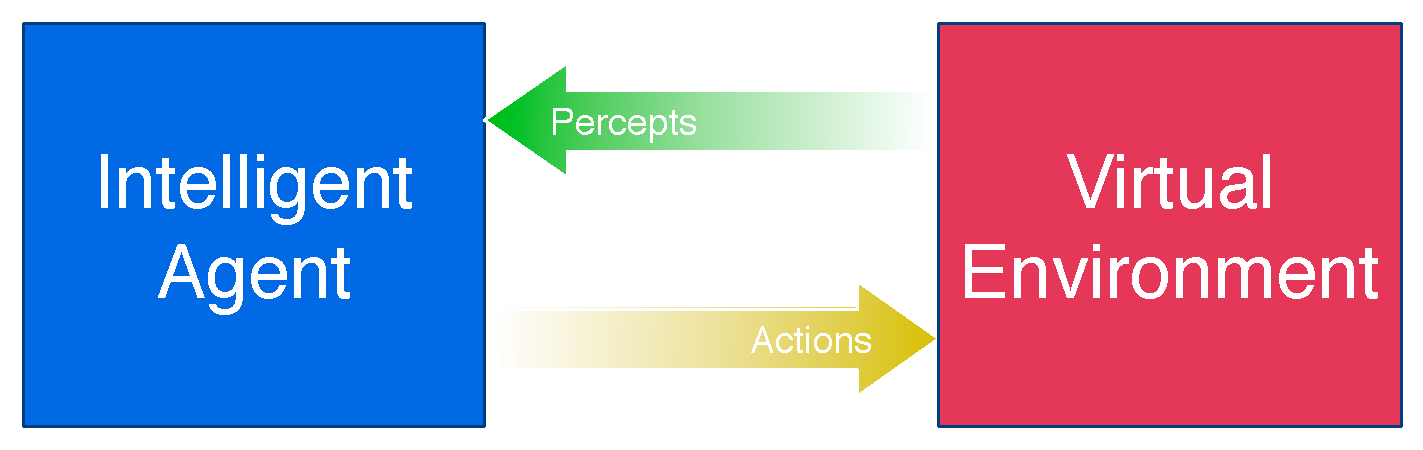
\includegraphics[width=10cm]{agent-env} 
\end{center} 
\end{frame} 

\begin{frame}{Situated Agents} 
\begin{center}
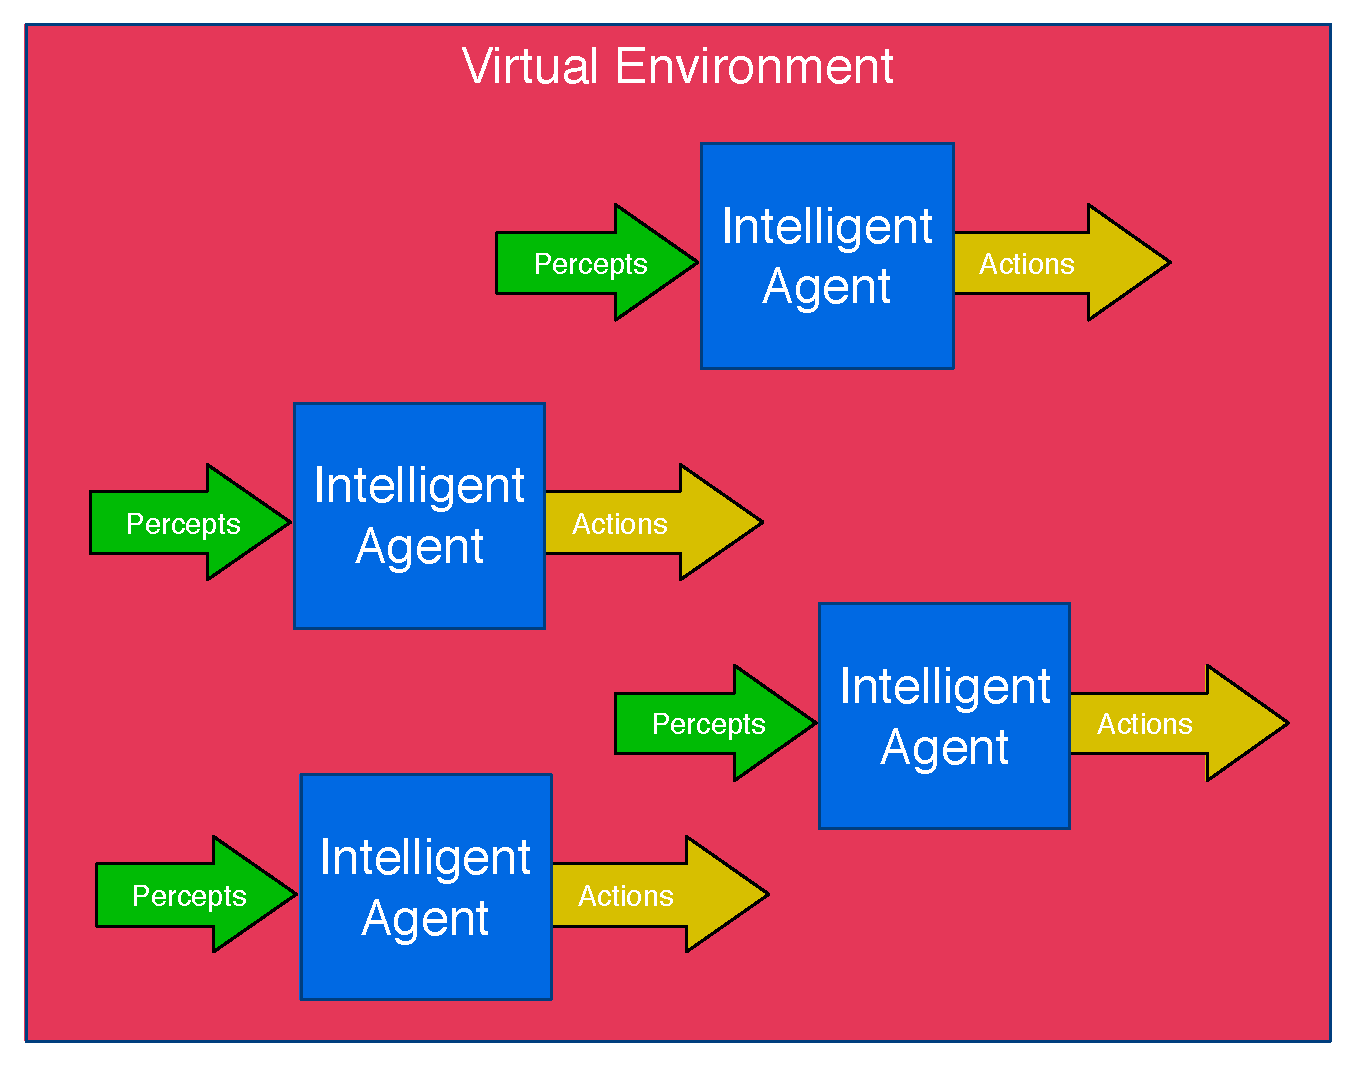
\includegraphics[width=10cm]{situated-agents} 
\end{center} 
\end{frame} 

\begin{frame}{Agents Processing Rendered Scenes} 
\begin{center}
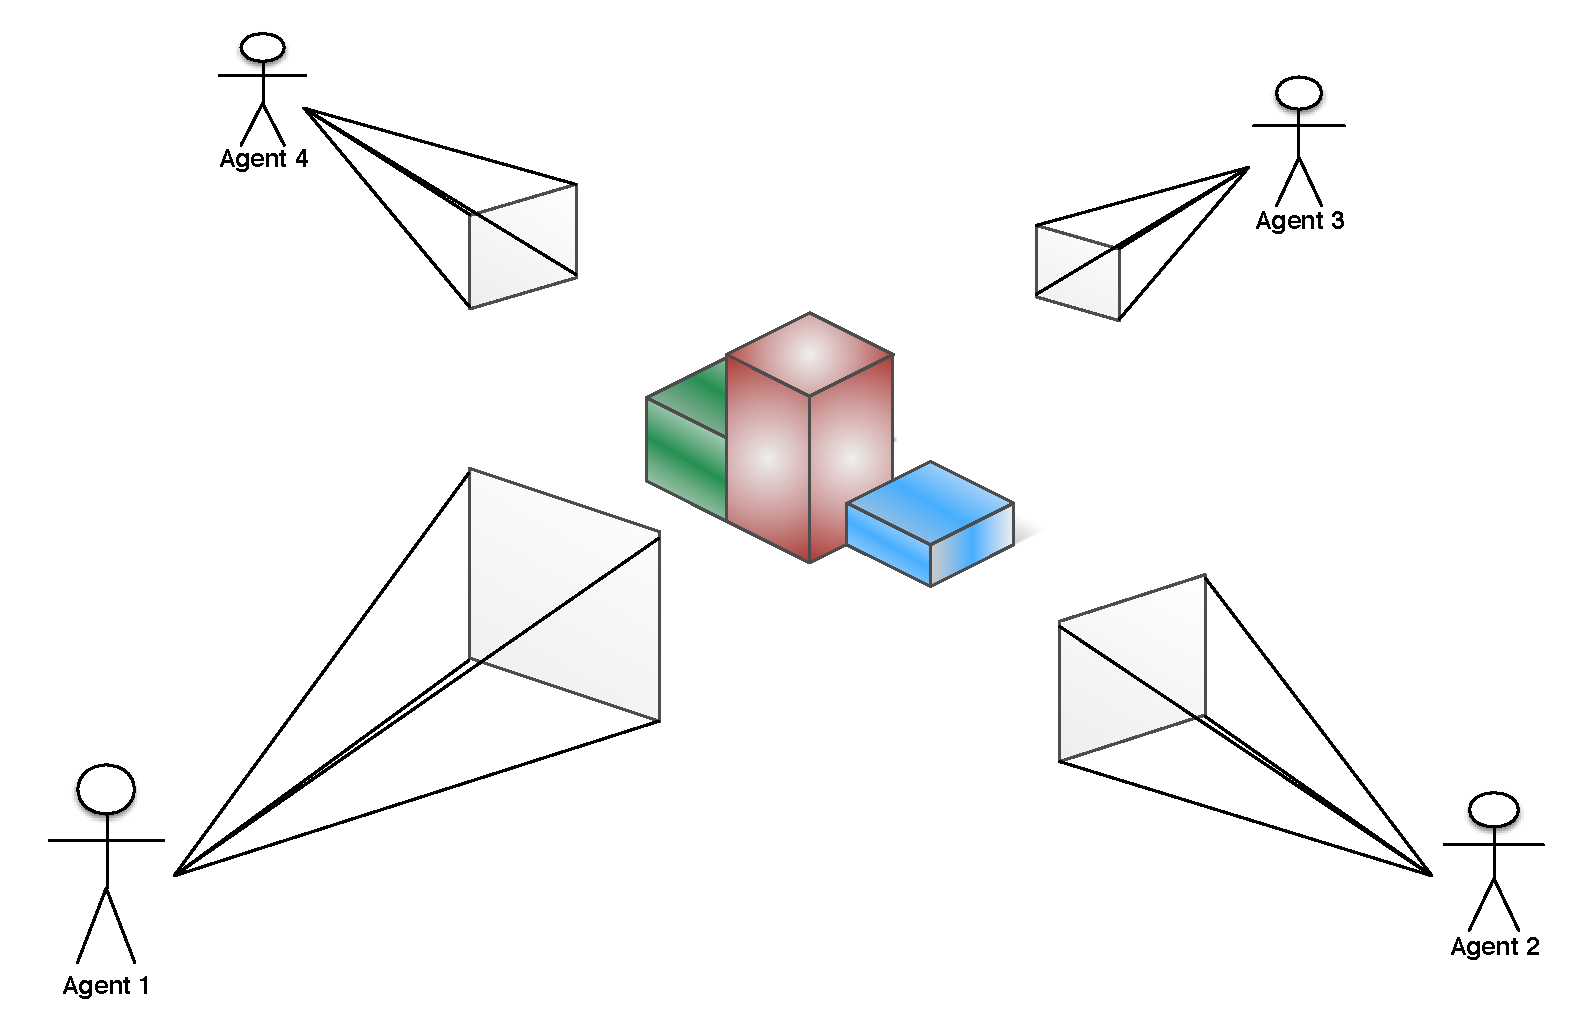
\includegraphics[width=9cm]{multi-agent-rendering} 
\end{center} 

Simpler solution: why not give Intelligent Agents access to the same
information that the graphical rendering engine receives?
\end{frame} 

\begin{frame}[fragile]{Data Structures for Graphical Rendering (Pseudo-Code)} 
    \begin{mdframed}[style=code2]
        \lstinputlisting{object.py} 
    \end{mdframed} 
\end{frame} 

\begin{frame}{Scene Graph}
\begin{itemize} 
\item A data structure representing the virtual world being rendered.
\item Is a \textbf{structured} representation of the world.
\item Can be any data structure but is typically a \emph{Directed Acyclic Graph} (DAG).
\item Often are represented as trees (special type of Directed Acyclic Graph). 
\item Scene graphs are made up of a variety of nodes (geometry/objects,
transformations, cameras, lighting, textures, materials etc.) 
\item A structured set of instructions to the rendering engine on how to render
the world~\footnote{OpenSceneGraph, X3D, Java3D, OpenInventor and VRML are examples
of scene graph libraries}. 
\end{itemize} 
\end{frame} 

\lstset{escapechar=@,style=json}
\begin{frame}{Scene Graph Editor Examples}
\begin{columns}[t] 
\column{0.5\textwidth} 
\begin{center} 
FX Composer [1] \\[0.1cm] 
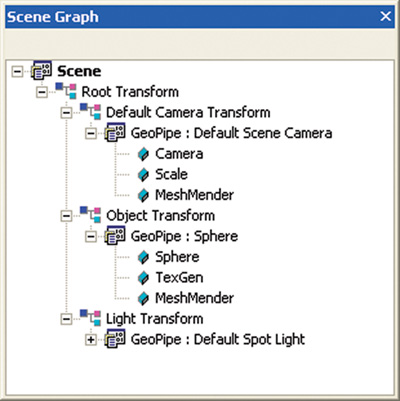
\includegraphics[width=5cm]{scene-graph-fxcomposer} 
\end{center} 
\column{0.5\textwidth} 
\begin{center}  
OSG Edit [2] \\[0.1cm] 
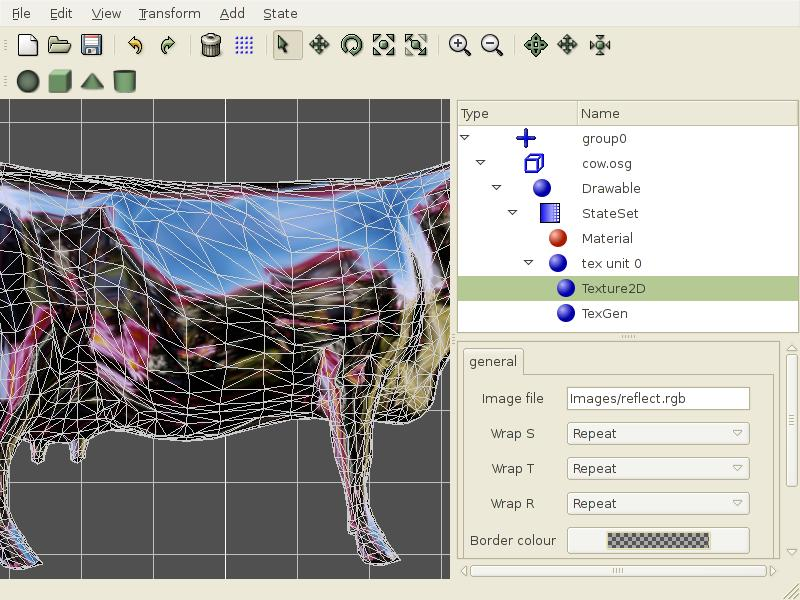
\includegraphics[width=5cm]{scene-graph-osgedit} 
\end{center} 
\end{columns} 
\small
\begin{itemize} 
\item [1] \url{http://http.developer.nvidia.com/GPUGems/gpugems_ch31.html} 
\item [2] \url{http://http://osgedit.sourceforge.net/shots/osgedit-0.6.1.jpg} 
\end{itemize} 
\normalsize
\end{frame} 

\begin{frame}{Scene Graphs and Intelligent Agents} 
\begin{itemize}
    \item A scene graph is a structured representation of the virtual environment..
\end{itemize} 
\begin{block}{Question}
Can intelligent agents interact with a scene graph?
\end{block} 
\pause
\begin{block}{Short Answer}
Sure... we could add labels/tags/annotations on the nodes in a scene graph
which contain information relevant to our Intelligent Agents. 
\end{block} 
\pause
\begin{block}{Long Answer} 
Sure... but there are bunch of potential issues and limitations...
\end{block} 

\end{frame} 

\begin{frame}{Example: Football Game} 
Let's start to label a scene graph from a virtual environment with labels that
could be useful to an Intelligent Agent (or NPC) playing the game.
\begin{center}
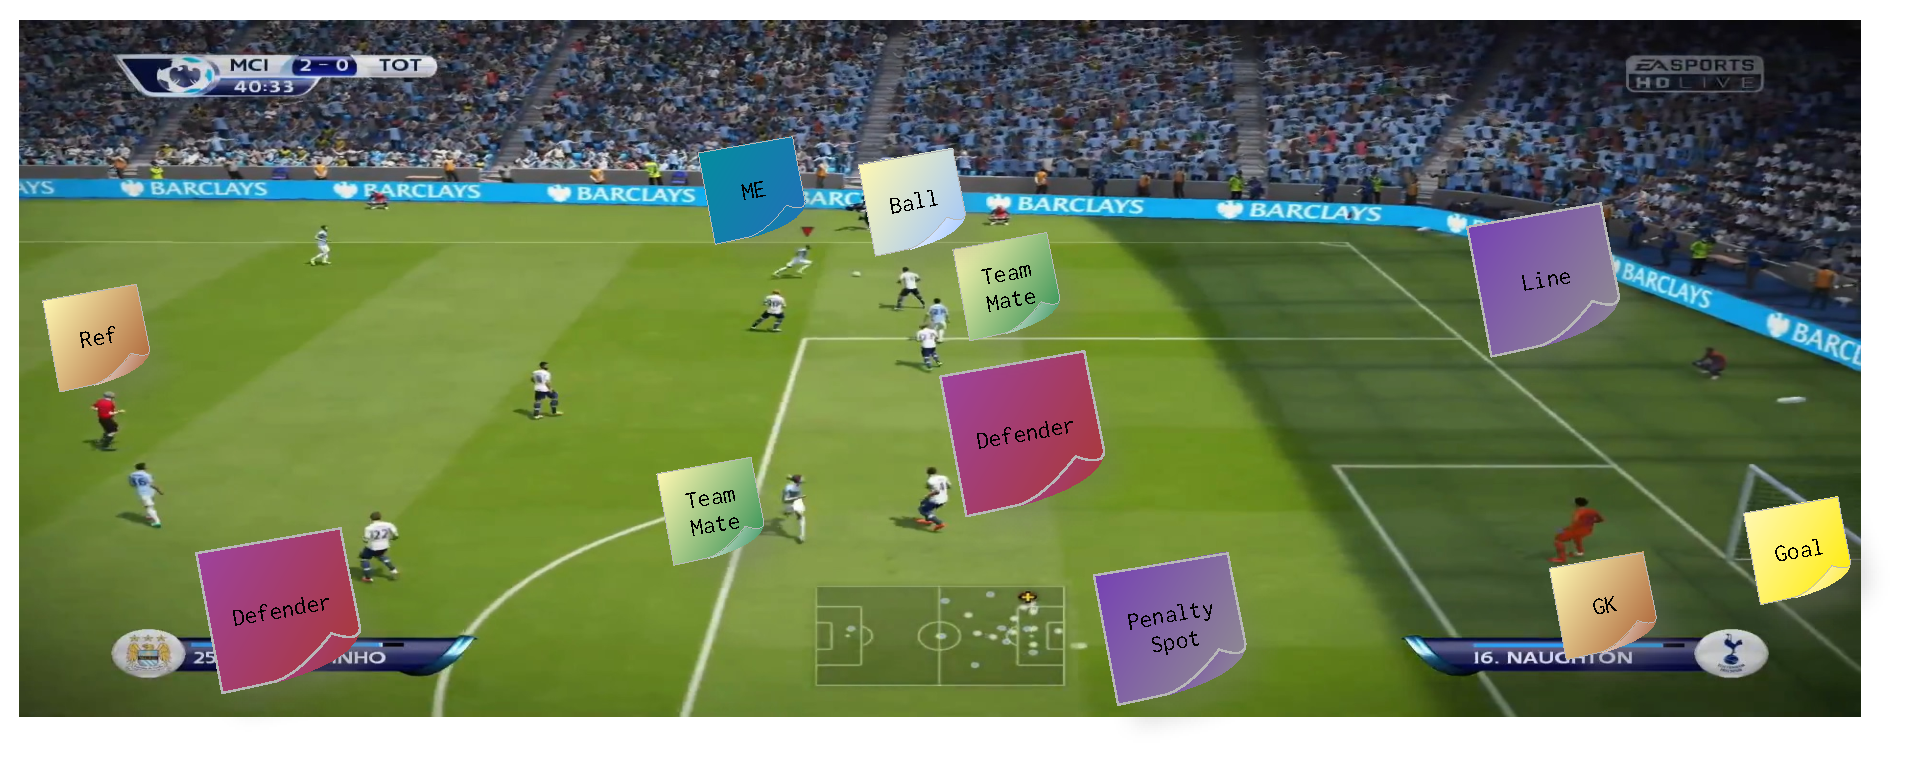
\includegraphics[width=\textwidth]{fifa-labels} 
\end{center}
Base image, screenshot from Electronic Arts FIFA 15.
\end{frame} 

\begin{frame}{Some Issues to Consider...} 
\begin{itemize} 
\item What if the label in the scene graph is different for different agents?
\item What if the labels need to be dynamic?  
\item What if we want to reason about something that isn't captured in the scene graph?
\end{itemize} 
\pause
\begin{block}{Conclusions}  
\begin{itemize} 
    \item Adding labels, tags or annotations that are useful to an Intelligent
    Agent is a first step to designing a virtual environment that is AI
    friendly.
    \item However, using a representation that was designed for a renderering
    engine instead of an AI engine isn't really ideal.
\end{itemize} 
\end{block} 
\end{frame} 

\begin{frame}{Multi-Modal Virtual Environments} 
\begin{center}
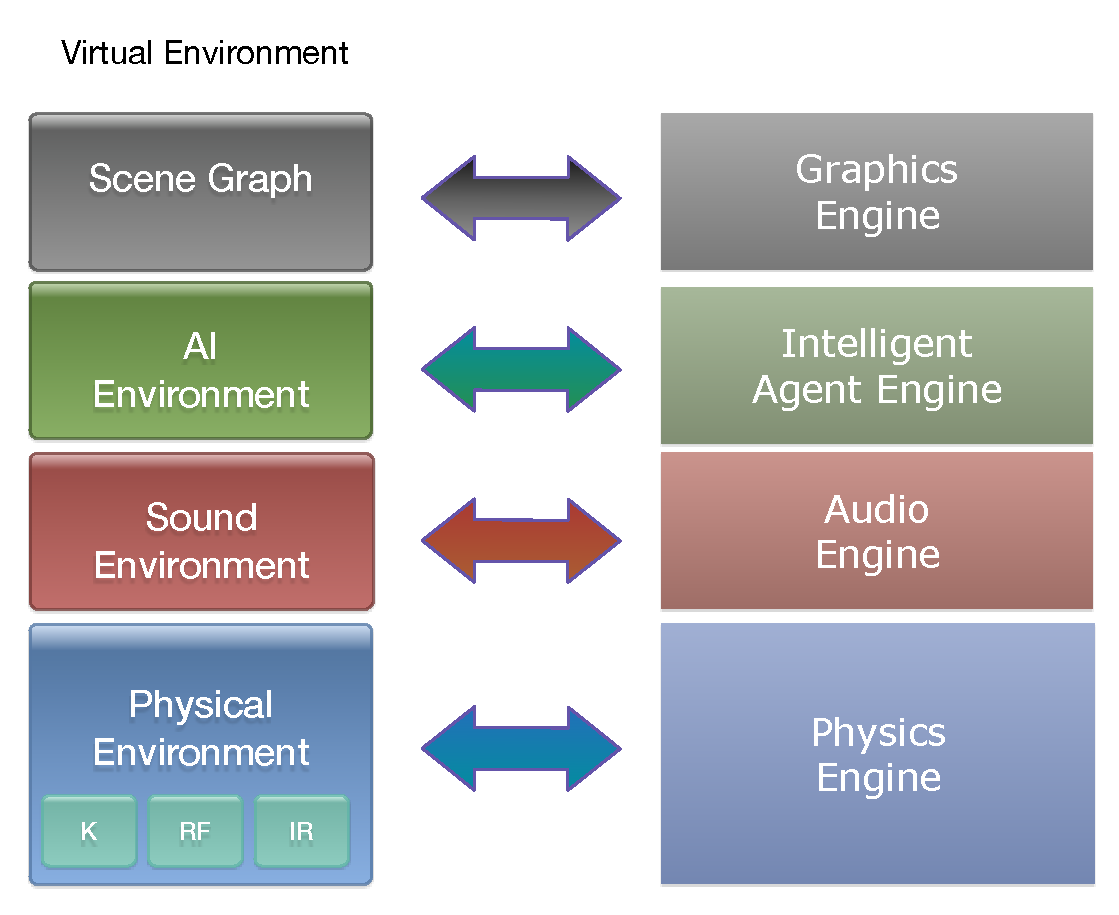
\includegraphics[width=8cm]{multi-modal} 
\end{center} 
\footnote{Compare w/ HTML, CSS, XML}
\end{frame} 

\begin{frame}{Example: Quake III} 
\begin{center}
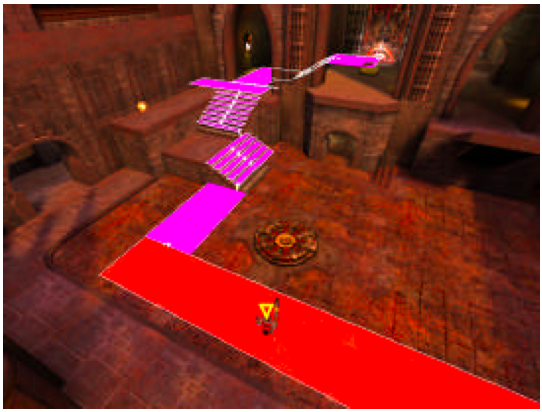
\includegraphics[width=4cm]{q3-route} \\
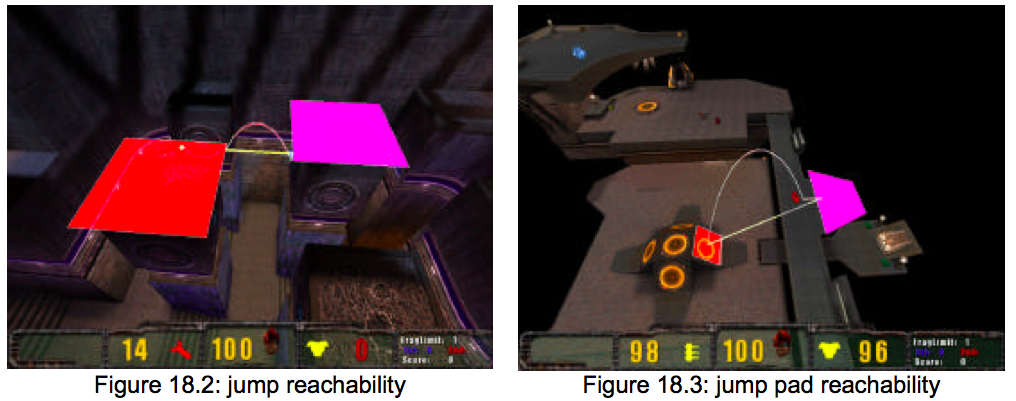
\includegraphics[width=10cm]{q3-annotations} 
\end{center} 
\tiny
\emph{Source: The Quake III Arena Bot by J.M.P. van Waveren (Masters Thesis 2001)}
\normalsize
\end{frame} 

\begin{frame}{Example: Killzone 3} 
\begin{center} 
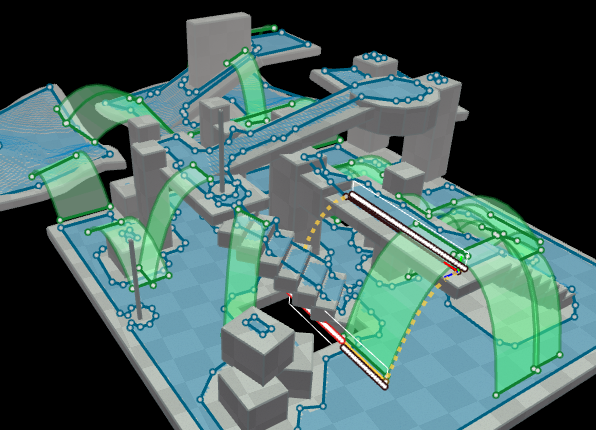
\includegraphics[width=8cm]{killzone3.png} 
\end{center} 
\tiny
\emph{Source: Auto Annotations in Killzone 3 by Mikko Mononen (2011 Paris
Game/AI Conference
\url{http://digestingduck.blogspot.com.au/2011/07/paris-gameai-conference-2011-slides-and.html}} 
\normalsize
\end{frame} 

\begin{frame}{Example: Halo 2} 
\begin{center} 
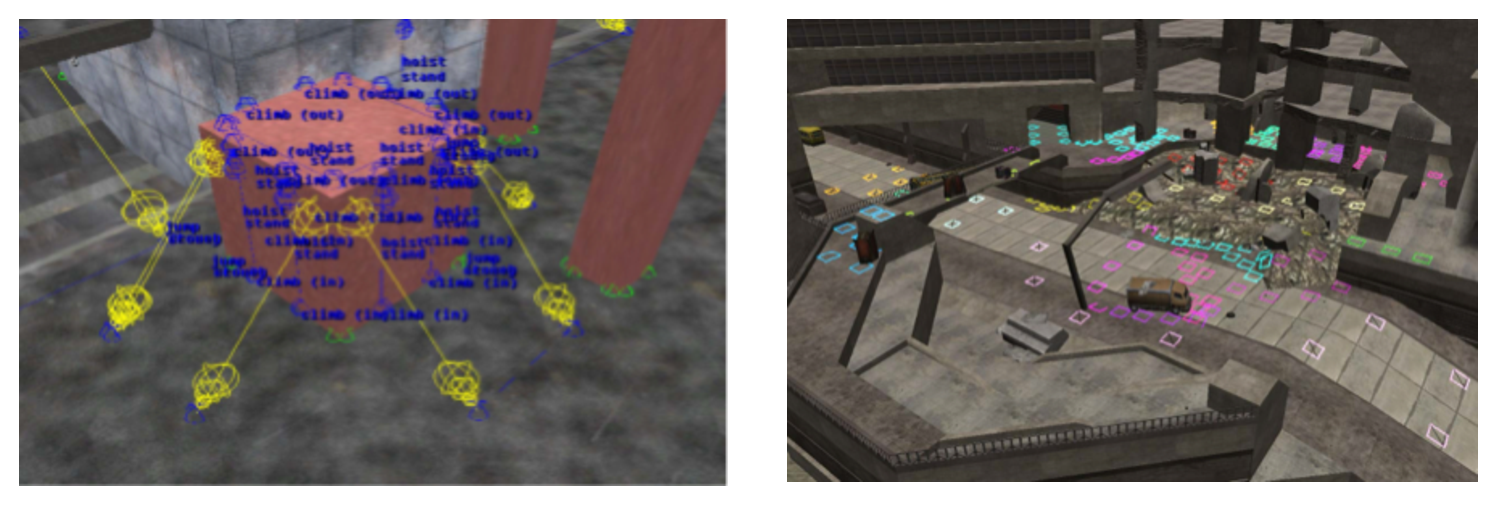
\includegraphics[width=10cm]{halo} 
\end{center} 
\tiny
\emph{Source: Dude, Where's My Warthog: From Pathfinding to General Spatial
Competence by Damian Isla, Bungie Studios. Proceedings of the first Artificial
Intelligence and Interactive Digital Entertainment Conference \\[1cm] 
\url{http://www.aaai.org/Library/AIIDE/aiide05contents.php} \\
\url{http://slideplayer.us/slide/686014/ } }
\normalsize
\end{frame} 

\begin{frame}{Desirable Characteristics of an Agent/AI Environment} 
If we are going to annotate our virtual environment with labels, tags
or annotations that intelligents agents can perceive, reason about
and take actions with respect to, it would be good if they were...
\begin{itemize} 
    \item Static 
    \item Dynamic
    \item Observer Tailored
    \item Relational 
    \item Action Oriented
    \item Intention/Goal Oriented
    \item Introspective
    \item Meaningful
    \item Context Sensitive
\end{itemize} 
\end{frame} 

\begin{frame}{Ecological Psychology} 
The study of how humans and animals interact with the environment they are
situated in. 
\begin{block}{Ecology} 
Ecology = Environment + Humans/Animals + Interaction 
\end{block} 
\begin{block}{Virtual Ecology} 
Virtual Ecology = Virtual Environment + Intelligent Agents + Interaction 
\end{block} 
\pause
\begin{itemize} 
\item A Multi-Agent Simulation or a Video Game is an example of a virtual ecology. 
\item Designing one of these systems involves designing a virtual ecology. 
\end{itemize} 

\end{frame} 

\begin{frame}{Affordance Theory} 
One of the key ideas in Ecological Psychology is the Theory of Affordances.
\begin{block}{Affordances} 
Affordances are the action possibilities an environment provides an agent.
\end{block} 
\pause
\begin{block}{J.J. Gibson's Definition} 
\emph{The affordances of the environment are what it offers the animal, what it
provides or furnishes, either for good or ill.} 
\end{block} 
\pause 
\begin{block}{Direct Perception} 
Gibson claimed that affordances (action possibilities) are directly perceivable
by humans and animals in the environment. 
\end{block} 
\end{frame} 

\begin{frame}{Affordances in Interaction Design} 
Affordance theory is important in the design of many things...
\begin{itemize}
    \item Everyday things (electronics, furniture, vehicles..)
    \item Human Computer Interfaces (e.g. Graphical User Interfaces). 
    \item Control panels for industrial processes and equipment.
\end{itemize} 
The affordances provided by a well designed object are obvious.
\end{frame} 

\begin{frame}{Affordances, Intelligent Agents and Virtual Environments} 
\begin{itemize} 
    \item One way to think about agent-environment interaction.
    \item Provide a mechanism for better situating intelligent agents in a
    virtual environment
    \item Allows for an agent to directly perceive the actions available to it
    (potentially without undertaking significant reasoning)
    \item Satisfy the desirable criteria for agent-environment interaction...
    \item Affordances are dynamic, tailored and context sensitive,
    intention/goal oriented and of course action oriented.
\end{itemize} 
\end{frame} 

\begin{frame}{Wrap Up} 
\begin{itemize} 
    \item Designing Intelligent Agents needs to be done in conjunction with the
    design of the virtual environment.
    \item Adapting existing environments (like scene graphs) for AI purposes
    can work in some cases put potentially doesn't scale. 
    \item Real environments are inherently multi-modal and hence so are the
    virtual environments we design. 
    \item Affordances are a good way to help you think about how to design a
    virtual ecology.
\end{itemize} 
\end{frame} 

\end{document} 


